% ACM manuscript layout for an independently distributed technical report.
\documentclass[manuscript,screen,nonacm]{acmart}
\setcopyright{none}
\settopmatter{printacmref=false,printccs=false}
\acmDOI{}
\acmISBN{}
\usepackage{longtable,booktabs,array,calc}
\usepackage{xurl}
\usepackage{fvextra}
\DefineVerbatimEnvironment{verbatim}{Verbatim}{breaklines=true,fontsize=\small}
\usepackage{tikz}
\usetikzlibrary{positioning}
\providecommand{\tightlist}{\setlength{\itemsep}{0pt}\setlength{\parskip}{0pt}}
\providecommand{\passthrough}[1]{#1}
\providecommand{\pandocbounded}[1]{#1}
\begin{document}
\title{AFFECTOR: Emotional Geometry Transfer through Transformer Activation
Steering}
\author{William Taggart}
\affiliation{\department{Modern and Classical Languages and Literatures}
\institution{Virginia Tech}\city{Blacksburg}\state{Virginia}\country{USA}}
\email{wtaggart@vt.edu}
\subtitle{Technical report; ACM manuscript edition, November 13, 2026}
\begin{abstract}
AFFECTOR is an experimental macOS application for transforming writing
according to emotional trajectories generated by Emotional Atlas or
authored directly by a user. It implements two distinct transformation
paths: local hidden-state intervention in a frozen Qwen3.5-0.8B model,
and prompt-guided rewriting through OpenAI or Virginia Tech Advanced
Research Computing (VT ARC) APIs. The local method converts
three-dimensional emotional coordinates into coefficients over
contrastively estimated activation vectors. A bounded perturbation
modifies both the feed-forward input and residual path at selected
transformer blocks. Independent assessment compares original and revised
passages with the requested coordinates using the Emotional Atlas
scoring prompt and validation rules. The application supports portable
geometry files, editable module weights, text document import/export,
checkpointing, and continuation after individual failures. Tests
establish several implementation properties, including zero-strength
output equivalence and hook cleanup. They do not establish reliable
emotional shape transfer, semantic preservation, or multilingual
effectiveness.
\end{abstract}
\keywords{activation steering, emotional text generation, transformer models, controllable generation}
\maketitle
\section{Literature review: activation steering and
emotion}\label{literature-review-activation-steering-and-emotion}

This focused review covers twelve papers, emphasizing 2025-2026 research
and retaining two methodological foundations. Titles, author lists,
version histories, and the claims summarized here were checked against
arXiv records and the corresponding paper text on November 13, 2026. The
cited versions are fixed below; availability on arXiv alone does not
establish peer review. The implications for this project are research
motivations, not evidence that its implementation reproduces these
results.

\textbf{From activation differences to behavioral control.} Activation
steering changes internal model states during inference while leaving
the backbone weights fixed. Turner et al.~derive intervention vectors
from contrasting prompts; Panickssery et al.~average differences across
positive and negative behavioral examples. These provide the
methodological basis for contrastive calibration, but do not validate a
particular emotional coordinate system or insertion site.
\citep{turner2023actadd}; \citep{panickssery2024caa}.

\textbf{Emotional expression and human judgment.} Wu et al.~relate model
emotion spaces to human valence/arousal judgments and report
concept-based steering across linguistic-cultural settings. Diallo et
al.~evaluate perceived emotional intensity and text quality with human
raters, finding that effects depend on emotion and steering strength.
Together they motivate separate measures of emotional movement and
readability. Their axes and numerical strengths cannot be assumed
equivalent to this project's inward/outward direction or RMS-scaled
controls. \citep{wu2025emotion}; \citep{diallo2026style}.

\textbf{Emotion can affect more than tone.} Sun et al.'s E-STEER uses
valence-arousal-dominance interventions to study reasoning, generation,
safety, and agent behavior, reporting non-monotonic relationships.
Jeong's small-model comparison reports both coherent emotional changes
and degeneration, including repetition, depending on extraction method
and architecture. These findings motivate reporting failed generations
alongside successes and testing strength sweeps rather than assuming
that larger perturbations improve emotional fit. Neither study
establishes an operating range for this implementation.
\citep{sun2026emotion}; \citep{jeong2026emotion}.

\textbf{Reading an emotion is different from controlling it.} Shu et
al.'s revised study identifies uneven causal organization of sparse
features across emotion categories and tests interventions for emotion
recognition. Wang et al.~show, in omni-modal models, that layers with
strong emotion-probing accuracy need not be the best intervention
layers. Recognition results therefore inform evaluator design, while
layer selection for rewriting still requires causal tests on generated
text. Neither finding licenses importing layer indices across
architectures. \citep{shu2026emotion}; \citep{wang2026readbest}.

\textbf{Multiple axes and adaptive control.} Ha et al.~find that
supportive-empathy directions are only partially separable: intervening
on one can shift other EPITOME proxy scores. Cui and Chen automate
vector extraction from labeled data, with task-dependent benefits.
Ferrando et al.~adapt intervention strength to context, studying the
balance between toxicity mitigation and retained utility. These
approaches motivate broader calibration, cross-axis tests, and future
adaptive control. The present coordinate mixture is not an
implementation of their learned selectors or context-dependent gates.
\citep{ha2026empathy}; \citep{cui2025pas}; \citep{ferrando2025dsas}.

\textbf{Evaluation must include costs as well as target effects.} Yang
et al.'s SteerScope evaluates steering efficacy jointly with side
effects, generalization, and data dependence. In its tested settings,
activation methods do not dominate prompt steering on the
efficacy/side-effect trade-off. For this project, the resulting
evaluation priorities are prompt-only and unsteered baselines, blinded
emotional and quality ratings, content-change assessment appropriate to
the rewrite style, and complete accounting of repetition, truncation,
and original-text fallbacks. This is an evaluation agenda, not a
completed benchmark. \citep{yang2026steerscope}.

\section{Scope and research
objective}\label{scope-and-research-objective}

The objective is to transfer an emotional progression from one text to
another while maintaining a recognizable connection to the target text's
subject and situation. Emotional Atlas supplies interpretive coordinates
for valence, emotional direction, and intensity. AFFECTOR treats these
as a trajectory indexed by progress through a document.

The implemented geometric object is this ordered trajectory. The system
does not fit a solid mesh, preserve a surface topology, or optimize a
four-dimensional volume. Its position coordinate supplies a temporal
ordering rather than a fourth independently steered emotional axis.
AFFECTOR can import Atlas object and evolution exports when their
metadata retains the underlying emotional analysis; bare mesh or PCA
coordinates are insufficient to recover the semantic axes.

The interface follows a monochrome visual style inspired by FENNEC and
includes persistent light/dark appearance settings. Native SwiftUI views
separate document transformation, geometry and weight editing, and
verification.

\section{System architecture}\label{system-architecture}


\begin{figure}[htbp]
\centering
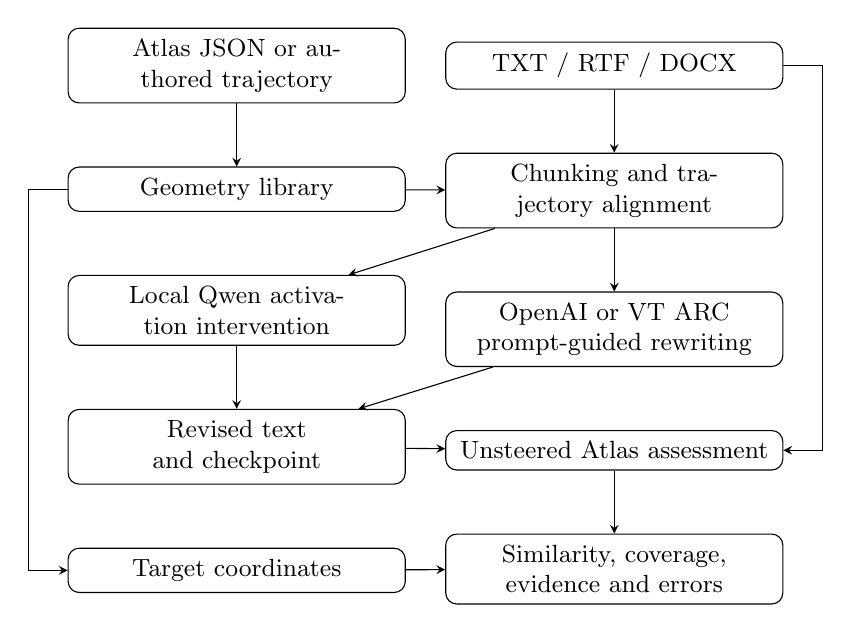
\begin{tikzpicture}[node distance=8mm and 5mm,
box/.style={draw,rounded corners,align=center,font=\small,text width=40mm,inner sep=4pt},
arr/.style={->,>=stealth}]
\node[box] (a) {Atlas JSON or authored trajectory};
\node[box,right=of a] (d) {TXT / RTF / DOCX};
\node[box,below=of a] (b) {Geometry library};
\node[box,below=of d] (e) {Chunking and trajectory alignment};
\node[box,below=of b] (f) {Local Qwen activation intervention};
\node[box,below=of e] (g) {OpenAI or VT ARC prompt-guided rewriting};
\node[box,below=of f] (h) {Revised text and checkpoint};
\node[box,below=of g] (i) {Unsteered Atlas assessment};
\node[box,below=of h] (j) {Target coordinates};
\node[box,below=of i] (k) {Similarity, coverage, evidence and errors};
\draw[arr] (a)--(b); \draw[arr] (d)--(e); \draw[arr] (b)--(e);
\draw[arr] (e)--(f); \draw[arr] (e)--(g);
\draw[arr] (f)--(h); \draw[arr] (g)--(h); \draw[arr] (h)--(i);
\draw[arr] (d.east)--++(5mm,0)|-(i.east);
\draw[arr] (b.west)--++(-5mm,0)|-(j.west);
\draw[arr] (i)--(k); \draw[arr] (j)--(k);
\end{tikzpicture}
\caption{Generation and independent assessment paths.}
\Description{Geometry and input feed local or hosted rewriting. Original and revised texts are assessed and compared with target coordinates.}
\end{figure}


A private JSON-lines subprocess bridge connects the native application
to the Python engine. No local web server is required. The bridge
serializes long-running operations; generation and assessment execute
outside the UI thread. The local model uses PyTorch on Apple's MPS
device when available, with CPU fallback. The packaged development app
includes its interpreter, libraries and model. The public source
repository excludes that large runtime and the application bundle.

Key implementation files are:

{ % do not increment counter
\begin{longtable}[]{@{}
  >{\raggedright\arraybackslash}p{(\linewidth - 2\tabcolsep) * \real{0.5000}}
  >{\raggedright\arraybackslash}p{(\linewidth - 2\tabcolsep) * \real{0.5000}}@{}}
\toprule\noalign{}
\begin{minipage}[b]{\linewidth}\raggedright
Component
\end{minipage} & \begin{minipage}[b]{\linewidth}\raggedright
Source
\end{minipage} \\
\midrule\noalign{}
\endhead
\bottomrule\noalign{}
\endlastfoot
Native interface and appearance &
\href{https://github.com/FL2744/AFFECTOR/blob/main/macos/Affector.swift}{\nolinkurl{macos/Affector.swift}} \\
Operation orchestration and checkpoints &
\href{https://github.com/FL2744/AFFECTOR/blob/main/engine/bridge.py}{\nolinkurl{engine/bridge.py}} \\
Geometry validation, interpolation and library &
\href{https://github.com/FL2744/AFFECTOR/blob/main/engine/geometry.py}{\nolinkurl{engine/geometry.py}} \\
Calibration, activation module and model hooks &
\href{https://github.com/FL2744/AFFECTOR/blob/main/engine/steering.py}{\nolinkurl{engine/steering.py}} \\
API requests and coordinate comparison &
\href{https://github.com/FL2744/AFFECTOR/blob/main/engine/providers.py}{\nolinkurl{engine/providers.py}} \\
Atlas scoring prompt, schema and validation &
\href{https://github.com/FL2744/AFFECTOR/blob/main/engine/atlas_analysis.py}{\nolinkurl{engine/atlas_analysis.py}} \\
Document conversion and chunk assembly &
\href{https://github.com/FL2744/AFFECTOR/blob/main/engine/documents.py}{\nolinkurl{engine/documents.py}} \\
\end{longtable}
}

\section{Emotional representation and
alignment}\label{emotional-representation-and-alignment}

A geometry stores points \((t,v,d,i)\) with position \(t\in[0,1]\),
valence \(v\in[-1,1]\), direction \(d\in[-1,1]\), and intensity
\(i\in[0,1]\). Negative direction represents inward/self-focused
emotion; positive direction represents emotion directed toward others or
the world. Direction is not synonymous with positive or negative
valence.

The steering coordinate uses the Atlas plot convention:

\[c(t)=(v(t),d(t),2i(t)-1).\]

Coordinates are linearly interpolated between stored points, with
endpoints clamped. Atlas positions with unsupported direction are
omitted rather than assigned a fabricated direction. The remaining
trajectory interpolates across those gaps, a limitation recorded in
import provenance.

Documents are divided into chunks of at most 700 characters, preferring
available whitespace boundaries. Given a chunk's original character
offsets \(a,b\) and total input length \(N\), its trajectory position is
\((a+b)/(2N)\). The target remains constant while that chunk is
generated. No token-level progression through the source trajectory
occurs within a chunk. Adjacent chunks are rewritten independently;
neighboring document text is not supplied as a continuity context.

\section{Contrastive activation
calibration}\label{contrastive-activation-calibration}

The local backend uses \nolinkurl{Qwen/Qwen3.5-0.8B}, pinned to revision
\nolinkurl{2fc06364715b967f1860aea9cf38778875588b17}. The text stack has 24
blocks and hidden width 1,024. The engine uses float32, eager attention,
frozen base parameters, inference mode, and a chat template with
thinking disabled. Model architecture and upstream licensing are
described in the
\href{https://huggingface.co/Qwen/Qwen3.5-0.8B}{official model card}.

Calibration uses twelve manually authored English contrast pairs: four
per emotional axis. These contrast unpleasant/pleasant affect,
inward/outward focus, and low/high intensity. Every member is processed
under a fixed instruction to continue in the same emotional voice,
producing 24 forward passes. At each selected layer, the code captures
the final prompt position immediately before the post-attention
normalization feeding the feed-forward network. Because a generation
prefix is appended, the capture is from the chat-formatted final
position, not an average of passage-token activations.

For layer \(\ell\) and axis \(j\), the raw direction is:

\[u_{\ell,j}=\frac{1}{4}\sum_{k=1}^{4}(h^+_{\ell,j,k}-h^-_{\ell,j,k}).\]

It is normalized using:

\[b_{\ell,j}=\frac{u_{\ell,j}}{\max(\operatorname{RMS}(u_{\ell,j}),10^{-8})},\qquad
\operatorname{RMS}(x)=\sqrt{\frac{1}{1024}\sum_{r=1}^{1024}x_r^2}.\]

The three directions form a matrix
\(B_\ell\in\mathbb{R}^{3\times1024}\). These are the editable module
weights. Default layers are 8, 16 and 23, indexed from zero, with
respective weights 1, 1 and 0.5. Geometry files preserve the matrices,
calibration pairs, model revision and runtime identity. Incompatible
identities are rejected at hook installation.

There is no backpropagation, supervised regression against Atlas scores,
orthogonalization, or outcome-driven selection of the directions. The
pairs can confound their intended axis with emotional category, subject
matter or other linguistic changes. Repeating the same deterministic
calibration does not constitute learning from a user's document.

\section{Steering coefficients, strength, inertia and
budget}\label{steering-coefficients-strength-inertia-and-budget}

For each axis, activation temperature \(T\) reshapes the target
coefficient:

\[a_j=\operatorname{sign}(c_j)|c_j|^{1/T}m_j.\]

The mask \(m\) keeps axes in descending order of \(|c_j|^{1/T}\).
Selection stops after activation top-k axes or when the cumulative
selected magnitude reaches the requested activation mass fraction. The
threshold-crossing axis is included. These controls act on three
emotional axes, not vocabulary tokens, and retained coefficients are not
renormalized. Defaults \(T=1\), top-k \(=3\), mass \(=1\) preserve all
target coefficients.

At a selected layer and decoding step, let \(h\) be the current
final-token state after the attention portion of the block. The raw
perturbation is:

\[r_{\ell,n}=s\,w_\ell\operatorname{RMS}(h_{\ell,n})(aB_\ell),\]

where \(s\) is strength and \(w_\ell\) is the layer weight. Default
strength is 0.12.

For inertia \(\rho\), the first step uses \(\tilde\delta=r\). Later
steps use:

\[\tilde\delta_{\ell,n}=\rho\delta_{\ell,n-1}+(1-\rho)r_{\ell,n}.\]

With budget \(\beta\), the applied perturbation is:

\[\delta_{\ell,n}=\tilde\delta_{\ell,n}
\min\left(1,\frac{\beta\operatorname{RMS}(h_{\ell,n})}{\max(\operatorname{RMS}(\tilde\delta_{\ell,n}),10^{-12})}\right).\]

The previous applied, already capped perturbation is retained for the
next step. Inertia and budget both default to 0.20. Module instances are
recreated per chunk, so inertia does not carry across chunks. Zero
strength, zero budget or zero layer weight returns an exactly zero
perturbation.

Budget is a per-layer bound on vector RMS, not a bound on each
component, token probabilities, downstream model amplification, or
percentage of text changed. Inertia smooths numerical adjustments across
decoding steps; because the chunk target is constant, it primarily
smooths changes driven by hidden-state scale.

\section{Transformer insertion and relation to
LAMP-Qwen}\label{transformer-insertion-and-relation-to-lamp-qwen}

The feed-forward portion of the unmodified block has the residual form:

\[y=h+\operatorname{FFN}(\operatorname{Norm}(h)).\]

AFFECTOR implements:

\[\boxed{y=(h+\delta)+\operatorname{FFN}(\operatorname{Norm}(h+\delta)).}\]

A forward pre-hook on \nolinkurl{post_attention_layernorm} adds the
perturbation to the feed-forward input. A forward hook on the decoder
block adds the same perturbation to the residual output. The second
addition supplies the residual change; it does not add a second
independent steering vector to the same branch. The implementation uses
the
\href{https://docs.pytorch.org/docs/2.15/generated/torch.nn.Module.html}{PyTorch
module hook interfaces}.

During prompt prefill, only the final position is modified. During
cached autoregressive decoding, the current position is modified at
every selected layer. Earlier prompt positions are not rewritten by
these hooks. All handles are removed in a \nolinkurl{finally} block,
including after exceptions.

This placement follows the pre-FFN and residual intervention used in the
local LAMP-Qwen prototype. The mechanism supplying the perturbation
differs: AFFECTOR has no associative recognition key, lexical trigger or
memory retrieval gate. Its trajectory coefficients continuously control
the selected layers. The present work does not reproduce or claim LAMP's
empirical findings.

The local rewriting prompt requests fluent prose retaining the main
subject and recognizable situation, while allowing changes in phrasing,
imagery and emotional expression. It contains no emotional coordinates.
Standard decoding temperature, top-p and top-k remain separate from
activation controls; temperature zero uses greedy decoding.

\section{A consequential limitation: target bias rather than error
correction}\label{a-consequential-limitation-target-bias-rather-than-error-correction}

The module mixes vectors using the absolute target coordinate. It does
not estimate the current chunk's emotional state before rewriting and
does not compute a target-minus-current emotional error.

Consequently, target valence zero produces no valence perturbation, even
if the input is strongly negative. Target intensity 0.5 becomes a zero
intensity coefficient and does not actively reduce or increase the input
toward moderate intensity. A larger strength can change the output
without making it closer to the target. There is no automatic
verification-driven revision loop.

The method is therefore an activation-bias prototype, not a demonstrated
inverse mapping from emotional geometry to language. This limitation is
central when interpreting weak or inconsistent transformations.

\section{API alternative}\label{api-alternative}

OpenAI rewriting uses Responses requests with \nolinkurl{store:false}; VT
ARC rewriting uses an OpenAI-compatible chat endpoint. API mode supplies
desired coordinates as instructions alongside the target passage. It
does not install a transformer module, expose hidden states, or apply
the local activation controls. The output-token limit applies to both
paths. Users choose model identifiers and supply their own credentials.

These adapters were implemented and exercised with mocked failures; live
authenticated provider calls were not part of the recorded validation.
Provider availability and model access depend on the user's account. API
keys are held in process memory and excluded from saved geometries,
checkpoints and reports. API passages leave the machine for the selected
provider; local mode uses the bundled model.

\section{Verification against Emotional
Atlas}\label{verification-against-emotional-atlas}

The evaluator is independently selectable. Original and revised chunks
are assessed without activation hooks using the Atlas prompt, schema,
direction consistency checks and exact-source evidence validation. These
checks establish response structure and traceability, not the
correctness of an emotional interpretation.

For a valid scored coordinate \(p\) and requested coordinate \(c\):

\[D(p,c)=\frac{\|p-c\|_2}{2\sqrt3},\qquad S(p,c)=1-D(p,c).\]

The denominator is the full diagonal of the Atlas cube \([-1,1]^3\).
Similarity is in \([0,1]\) and is not a probability. Per-axis absolute
errors are also exported, with intensity expressed on the scaled plot
axis. Summary improvement is the mean revised similarity minus the mean
original similarity, calculated only over paired valid assessments.
Coverage is paired valid chunks divided by all document chunks.

Failed assessments and unsupported directions are excluded rather than
replaced with zeros. Original-retained rewrites remain visible in the
report. The score measures target proximity, not semantic preservation,
factual accuracy, literary merit, or an independently established
psychological property. Use of the same small model for generation and
evaluation introduces correlated-error risk; an independent evaluator
can help but does not remove the interpretive nature of the coordinates.

\section{Failure handling, persistence and document
fidelity}\label{failure-handling-persistence-and-document-fidelity}

Each assessment receives one attempt. Invalid output, timeouts, API
failures and incidental interruptions are recorded at chunk/assessment
level, and the run proceeds. A failed rewrite retains the original
chunk. An explicit user Stop still cancels the run. Model
initialization, calibration, invalid geometry and checkpoint-storage
failures are run-level conditions rather than ordinary chunk failures.

Local generation has a 120-second budget checked between decoding steps.
This is not a hard interrupt of a blocking kernel or model
initialization. In-flight API calls can wait until their network timeout
before cancellation takes effect. Failed requests may already have
consumed provider usage.

Completed chunks are checkpointed through atomic JSON replacement. A
signature of input text, geometry, backend, model and sampling settings
controls reuse on resume. Geometry files and transfer files preserve
editable settings; transfer checkpoints include the full source and
output text and should be handled accordingly.

TXT, RTF and DOCX import/export support plain textual content. Rich
formatting, tracked changes and embedded media are not preserved.
Assembly preserves original inter-chunk separators, while rewritten
chunk contents can change. The application provides manual checkpoint
saving, geometry import/export/deletion and JSON report export.

\section{Validation and evidence}\label{validation-and-evidence}

On November 12, 2026, all \textbf{11 automated tests} passed. They cover
geometry import/validation, similarity endpoints, document round trips,
library operations, checkpoint reuse and credential exclusion,
failed-chunk continuation, explicit Stop, and single-attempt assessment
behavior. The transport tests cover connection, timeout, incidental
interruption and provider request errors. These tests are contained in
\href{https://github.com/FL2744/AFFECTOR/blob/main/tests}{\nolinkurl{tests}}.

A recorded real-model smoke test on MPS additionally checked:

\begin{itemize}
\tightlist
\item
  Identical greedy text with zero strength and without steering.
\item
  Nonzero hook injections during a steered rewrite.
\item
  Disabled gradients on all base model parameters.
\item
  Hook removal after generation.
\item
  Restoration of baseline output after steering.
\item
  Enforcement of the perturbation RMS budget.
\end{itemize}

For the synthetic kitchen-table letter passage, the baseline produced 69
tokens; a steered run at strength 0.25 and target \((0.8,0.5,0.5)\)
produced 29 tokens with 90 recorded layer injections and mean injected
RMS approximately 0.02768. The steered output introduced ``her heart
racing.'' These observations demonstrate a numerical intervention and an
output difference, not successful geometric matching.
\nolinkurl{activation_injections} counts nonzero layer-position
interventions, not emotionally changed words. No parameter hash
comparison was performed; the frozen-parameter test checks
\nolinkurl{requires_grad}, supplemented by baseline restoration.

The historical result is preserved in
\href{https://github.com/FL2744/AFFECTOR/blob/main/artifacts/model-smoke.json}{\nolinkurl{artifacts/model-smoke.json}}.
Its local assessment used the earlier two-attempt correction policy and
passed after correction. \textbf{It does not demonstrate success under
the current one-attempt policy.} The latest single-attempt behavior is
covered by dedicated regression tests. The stored calibration file has
default control settings; the smoke-test script explicitly changes
strength to 0.25 for its steered generation.

No held-out corpus study, multilingual benchmark, semantic-fidelity
evaluation, human rating study, or statistical comparison of steering
strengths has been completed. Runtime measurements are illustrative
single-machine observations, not performance guarantees. User
observations of weak transformation remain consistent with these
limitations.

\section{Reproduction, packaging and next
experiments}\label{reproduction-packaging-and-next-experiments}

The tested runtime uses Python 3.14, PyTorch 2.15.0 and Transformers
5.22.2. Complete dependency pins are in
\href{https://github.com/FL2744/AFFECTOR/blob/main/requirements-lock.txt}{\nolinkurl{requirements-lock.txt}}.
The native package targets Apple Silicon and macOS 26+. It is locally
ad-hoc signed and has not been notarized for public distribution.

The build script consumes an existing relocated runtime through
\nolinkurl{AFFECTOR_RUNTIME}; its development default points to the local
LAMP-Qwen application resources. It copies numerical libraries, model
files and dependency notices, not LAMP associative memories. A clean
machine must provide that runtime layout before using the script. The
repository is source and documentation, not a turnkey installer, and
contains neither the model checkpoint nor the packaged app.

Run the ordinary test suite with a Python environment matching the
dependency pins:

\begin{verbatim}
python -m unittest discover -s tests -p 'test_*.py' -v
\end{verbatim}

The real-model check additionally needs the pinned model cached locally,
discoverable through \nolinkurl{HF_HOME}, or supplied through
\nolinkurl{AFFECTOR_MODEL}:

\begin{verbatim}
python tests/model_smoke.py
\end{verbatim}

Priority follow-up experiments are to compare opposite targets under
fixed decoding; build larger, better-controlled contrast sets; fit
steering coefficients against measured Atlas outcomes; examine
layer-specific effects and axis interference; and test
target-minus-current corrections. Quality evaluation should report
coverage, negative results, semantic changes and uncertainty alongside
similarity improvement. These are proposed experiments, not implemented
capabilities.

\section{Implementation sources and
provenance}\label{implementation-sources-and-provenance}

\begin{enumerate}
\def\labelenumi{\arabic{enumi}.}
\tightlist
\item
  \href{https://github.com/FL2744/Emotional-Atlas}{Emotional Atlas
  source repository}: emotional coordinate framework and copied
  scoring/validation components. The retained MIT notice is
  \href{https://github.com/FL2744/AFFECTOR/blob/main/ATLAS_LICENSE}{\nolinkurl{ATLAS_LICENSE}}.
\item
  \href{https://huggingface.co/Qwen/Qwen3.5-0.8B}{Qwen3.5-0.8B official
  model card}: model specification and Apache-2.0 licensing. The
  implementation pins the revision listed above.
\item
  \href{https://docs.pytorch.org/docs/2.15/generated/torch.nn.Module.html}{PyTorch
  Module documentation}: forward and forward-pre hooks used to install
  the intervention.
\item
  LAMP-Qwen local prototype: architectural precedent for paired
  pre-FFN/residual intervention. Its recognition and memory mechanism is
  not included in AFFECTOR.
\item
  \href{https://l1001.vt.domains/fennec.html}{FENNEC}: interface styling
  reference.
\end{enumerate}

This report describes the implementation and recorded development
evidence available on the date above. It makes no claim of peer review
or validated emotional control.

\bibliographystyle{ACM-Reference-Format}
\bibliography{references}
\begin{samepage}
\section*{AI assistance disclosure}
This project was created with assistance from GPT-6 Astra and Codex. AI
tools supported software development, testing, and the drafting and
revision of this technical report. William Taggart is responsible for
the project's research decisions and the final software and
documentation. AI assistance does not constitute independent validation
of the implementation or its scientific claims; the validation evidence
and limitations are stated separately in this report.

\section*{Suggested citation}
William Taggart. 2026. AFFECTOR: Emotional Geometry Transfer through
Transformer Activation Steering. Technical report. Modern and Classical
Languages and Literatures, Virginia Tech. ACM manuscript edition,
November 13, 2026.
\url{https://github.com/FL2744/AFFECTOR/blob/main/docs/TECHNICAL_REPORT.md}

\end{samepage}
\end{document}
